%%%%%%%%%%%%%%%%%%%%%%% file template.tex %%%%%%%%%%%%%%%%%%%%%%%%%
%
% This is a general template file for the LaTeX package SVJour3
% for Springer journals.          Springer Heidelberg 2010/09/16
%
% Copy it to a new file with a new name and use it as the basis
% for your article. Delete % signs as needed.
%
% This template includes a few options for different layouts and
% content for various journals. Please consult a previous issue of
% your journal as needed.
%
%%%%%%%%%%%%%%%%%%%%%%%%%%%%%%%%%%%%%%%%%%%%%%%%%%%%%%%%%%%%%%%%%%%
%
% First comes an example EPS file -- just ignore it and
% proceed on the \documentclass line
% your LaTeX will extract the file if required
\begin{filecontents*}{example.eps}
%!PS-Adobe-3.0 EPSF-3.0
%%BoundingBox: 19 19 221 221
%%CreationDate: Mon Sep 29 1997
%%Creator: programmed by hand (JK)
%%EndComments
gsave
newpath
  20 20 moveto
  20 220 lineto
  220 220 lineto
  220 20 lineto
closepath
2 setlinewidth
gsave
  .4 setgray fill
grestore
stroke
grestore
\end{filecontents*}
%
\RequirePackage{fix-cm}
%
%\documentclass{svjour3}                     % onecolumn (standard format)
%\documentclass[smallcondensed]{svjour3}     % onecolumn (ditto)
%\documentclass[smallextended]{svjour3}       % onecolumn (second format)
\documentclass[twocolumn]{svjour3}          % twocolumn
%
\smartqed  % flush right qed marks, e.g. at end of proof
%
\usepackage{graphicx}
\usepackage{amssymb}
%
% \usepackage{mathptmx}      % use Times fonts if available on your TeX system
%
% insert here the call for the packages your document requires
%\usepackage{latexsym}
% etc.
%
% please place your own definitions here and don't use \def but
% \newcommand{}{}
%
% Insert the name of "your journal" with
% \journalname{myjournal}
%
\begin{document}

\title{Multifractal characterization and classification of bread crumb digital images%\thanks{Grants or other notes
%about the article that should go on the front page should be
%placed here. General acknowledgments should be placed at the end of the article.}
}
%\subtitle{Do you have a subtitle?\\ If so, write it here}

%\titlerunning{Short form of title}        % if too long for running head

\author{Rodrigo Baravalle         \and
        Claudio Delrieux \and
        Juan Carlos G\'omez
}

%\authorrunning{Short form of author list} % if too long for running head

\institute{Rodrigo Baravalle and Juan Carlos G\'omez \at
              Laboratorio de Sistemas Din\'amicos y Procesamiento de Informaci\'on \\
              FCEIA, Universidad Nacional de Rosario, - CIFASIS - CONICET \\
              Riobamba 250 bis, 2000, Rosario, Argentina. \\
              Tel.: +54-341-4237248 int. 301\\
              Fax: +54-341-4821772 int. 3\\
              \email{baravalle@cifasis-conicet.gov.ar}
           \and
           Claudio Delrieux \at
               DIEC, Universidad Nacional del Sur - IIIE-CONICET \\
               Avenida Col\'on 80 - Bah\'ia Blanca (8000FTN) \\
               Provincia de Buenos Aires - Rep\'ublica Argentina
}

\date{Received: date / Accepted: date}
% The correct dates will be entered by the editor


\maketitle

\begin{abstract}

An adequate model of bread crumb structure can be critical for understanding flow and transport
processes in bread, creating synthetic bread crumb images for photo-realistic rendering, and evaluating similarity of different bread crumbs.

In this article multifractal analysis, employing the multifractal spectrum (MFS), has been used to study the structure of the bread crumb in four varieties of breads ({\em baguette}, {\em lactal}, {\em bran}, and {\em sandwich}). The extracted dimensions could be used to discriminate among bread crumbs from different types. Also, high correlations were found between some of these parameters and the porosity, coarseness, and heterogeneity of the samples. These results demonstrate that the MFS is an appropriate tool for characterizing the internal structure of the bread crumb and thus may be used to establish important quality properties that it should have.


The MFS has shown to provide local and global image features that are both robust and low-dimensional. In this work we also apply the MFS for bread crumb classification based on color scans of slices of different bread types. Results show that MFS based classification is able to distinguish different bread crumbs with very high accuracy. The multifractal modeling of the bread crumb structure can be an efficient method for parameterizing and simulating the appearance of different bread crumbs.

\keywords{Fractal \and Multifractal \and Image analysis \and Image classification \and Bread crumb}
% \PACS{PACS code1 \and PACS code2 \and more}
% \subclass{MSC code1 \and MSC code2 \and more}
\end{abstract}

\section{Introduction}
\label{intro}
Among other important factors, the quality of a bread loaf is related to its crumb structure. Close examination of different slices reveals considerable variation in the cell size even within a single sample of the same bread type. 

Fractal and multifractal analysis of images have proved to capture useful properties of the underlying material being represented. These features have been successfully applied in different areas, such as medicine \cite{Andjelkovic2008,Yu2011} and texture classification \cite{Wendt2009}. Through several procedures, it is possible to obtain different Fractal Dimensions (FD), each of them capturing a different property of the material ({\em e.g.}, porosity, rugosity).

For each material, the results obtained in classification tasks and in the analysis of the data in the feature extraction process are useful in quality measurements of real samples and also in the validation of synthetic representations of them. In other words, these processes are useful to determine if a given image presents the observed features in that material, allowing to associate quality measure parameters to the material. In~\cite{Fan2006}, a quality bread crumb test based on Gabor filters was performed in that paper, obtaining good results. Nevertheless, a small database was used ($30$ images). In \cite{Gonzales2008} several fractal features were obtained for one type of bread, showing that a vector comprising them would be capable of obtaining key features of its crumb texture.

In this work we propose the application of the MFS \cite{Xu2006} to describe and discriminate among different bread types. One of the main features of the MFS is its bi-Lipschitz invariance \cite{bilipXXX}, which includes perspective transforms (viewpoint changes) and smooth texture surface deformations. It is shown that the MFS is also locally invariant to affine changes in illumination.

The proposed method is compared to other classifiers that uses state-of-the-art features for texture classification. The results of this feature extraction procedure show that the classifier is robust and presents good discrimination properties to distinguish between different types of bread and also non bread images. The objectives of this study were: (1) to evaluate if the MFS can be applied to characterize and discriminate the bread crumb structure from different bread types from digital images, and (2) to investigate the efectiveness of the method in the classification of these structures.

In section 2 the theory underlying fractal sets is introduced, and the materials and methods employed in this work are presented. In section 3 the results obtained in the characterization and classification  are shown and discussed. In section 4 the conclusions are summarized, and some possible future works are posed.


\section{Materials and Methods}
\label{sec:1}
\subsection{Fractals and Multifractals}
\label{sec:2}

The term {\em Fractal} was first employed by the mathematician Mandelbrot in \cite{Mandelbrot83}. Fractal objects have the property of self-similarity (the structure is repeated at different scales), and they are characterized by a non-integer dimension. Multifractal formalisms decompose structures into fractal sets, each of them characterized by a different FD. The result is a vector containing several FDs. The multifractal approach characterizes better the objects than the fractal one, since it captures more accurately variations in local regions.

%as required. Don't forget to give each section
%and subsection a unique label (see Sect.~\ref{sec:1}).
%\paragraph{Paragraph headings} Use paragraph headings as needed.
%\begin{equation}
%a^2+b^2=c^2
%\end{equation}

% For one-column wide figures use
%\begin{figure}
% Use the relevant command to insert your figure file.
% For example, with the graphicx package use
%  \includegraphics{example.eps}
% figure caption is below the figure
%\caption{Please write your figure caption here}
%\label{fig:1}       % Give a unique label
%\end{figure}
%
% For two-column wide figures use
%\begin{figure*}
% Use the relevant command to insert your figure file.
% For example, with the graphicx package use
%  \includegraphics[width=0.75\textwidth]{example.eps}
% figure caption is below the figure
%\caption{Please write your figure caption here}
%\label{fig:2}       % Give a unique label
%\end{figure*}
%
% For tables use
%\begin{table}
% table caption is above the table
%\caption{Please write your table caption here}
%\label{tab:1}       % Give a unique label
% For LaTeX tables use
%\begin{tabular}{lll}
%\hline\noalign{\smallskip}
%first & second & third  \\
%\noalign{\smallskip}\hline\noalign{\smallskip}
%number & number & number \\
%number & number & number \\
%\noalign{\smallskip}\hline
%\end{tabular}
%\end{table}

\subsubsection{Box dimension}
\label{sec:3}
Mathematical objects such as the Koch curve and the Sierpinsky triangle have exact self-similarity. Natural phenomena, on the other hand, is better described by statistical self-similarity. Box FD is a simplification of the Hausdorff (originally Minkowski - Bouligand) dimension for non strictly self-similar objects \cite{Peitgen2004}. Given a binarised image, it is subdivided in a grid of size $M\times M$ where the side of each box formed is $\epsilon$. If $N_{\epsilon}$ represents the amount of boxes that contains at least one pixel in the binarisation of the set for that $\epsilon$, then the box dimension  $D_{b}$ is defined as

\begin{equation}
D_{b} \triangleq \displaystyle\lim_{\epsilon \to 0}{\frac{\log(N_{\epsilon})}{\log (1/\epsilon)}}.
\label{eqn:1}
\end{equation}

The algorithm uses a binarised image and selects different values of $\epsilon$ in it, making a count of the boxes that contains pixels in each case (to avoid numerical instabilities, a mean of cases is computed, establishing different positions in the grid over the image). Finally, a linear regression adjustment is made with the obtained data, in the $\log-\log$ space, and the slope of the straight line is by definition the box dimension of the image. %In Fig. \ref{fig:1} an image of the bread type {\em salvado} is shown with its corresponding box dimension computation.


\subsection{Multifractal analysis}
\label{sec:4}
The fractal dimension is an exponent which relates the statistical self similarity of the object at different scales. On the one hand, deterministic fractals are characterized by one FD. They are called {\em monofractals} (for instance, Koch Curve, Sierpinsky triangle). On the other hand, {\em multifractals} \cite{Mandelbrot89} are characterized by a set of FDs. It is assumed that these structures are composed by different fractals coexisting simultaneously.

\subsubsection{MFS and the H\"older exponent}
\label{sec:5}
Informally, the way to proceed with multifractal analysis is to examine, in the limit, the local behavior of a measure $\mu$ at each point of the set under study. This means, to find the H\"older exponent $\alpha$ in that point. The {\em multifractal spectrum} $f(\alpha)$ is obtained applying this procedure to the entire set, in this case, an image.

Let $E$ be an structure divided in disjoint substructures $E_{i}$ of size $\epsilon$ in such a way that 

\begin{equation}
\displaystyle\bigcup_{i}E_{i} = E.
\end{equation}

Each substructure $E_{i}$ is characterized by a measure $\mu(E_{i})$. From the point of view of multifractal analysis, it is useful to define this value as a function of $\epsilon$, {\em i.e.}


\begin{equation}
\alpha_{i} = \frac{ln(\mu(E_{i}))}{ln(\epsilon)},
\label{eqn:eqn4}
\end{equation}
\noindent
and to take the limit when $\epsilon$ tends to $0$. The limit represents the value of the H\"older exponent at a point in the structure, that is

\begin{equation}
\alpha = \lim_{\epsilon\to0}{\alpha_{i}}.
\label{eqn:eqn5}
\end{equation}

The exponent characterizes the local regularity of the structure at a point. To obtain a global characterization of its regularity it is necessary to obtain the distribution of $\alpha$ in $E$. For this, a counting $N_{\epsilon}$ must be done for each $\alpha_{i}$, related to the value of $\epsilon$, {\em i.e.}

\begin{equation}
f_{\epsilon}(\alpha_{i}) = - \frac{ln(N_{\epsilon}(\alpha_{i}))}{ln(\epsilon)}.
\label{eqn:eqn6}
\end{equation}

When $\epsilon$ tends to $0$, the limiting value is the FD of the structure $E$ characterized by $\alpha$, the Hausdorff dimension of the $\alpha$ distribution, also known as the {\em multifractal spectrum} $f(\alpha)$ \cite{Silvetti2010}, {\em i.e.}

\begin{equation}
f(\alpha) = \lim_{\epsilon\to0}{f_{\epsilon}(\alpha)}.
\label{eqn:eqn7}
\end{equation}

\subsubsection{Procedure for the MFS}
As illustrated in \cite{Xu2006}, the domain is partitioned into non-overlapping boxes of length $r$. The $q$-th moment of a measure $\mu$ is defined as
\begin{equation}
M_{r}(q) = \sum{\mu(B(x,r))^{q}},
\label{eqn:eqn8}
\end{equation}

where the sum is over the $r$ mesh squares for which $\mu(B(x,r)) > 0$. To denote the power law behavior of $M_{r}(q)$, $\beta(q)$ is defined as a straight line fit of the values $M_{r}(q)$ with respect to $r$, for $r$ in $1,..,n$. It is shown in \cite{Falconer97}, that the MFS and $\beta(q)$ are related to each other by a Legendre transform as

\begin{equation}
f(\alpha(q)) = q \alpha(q) - \beta(q),
\label{eqn:eqn9}
\end{equation}

where

\begin{equation}
\alpha(q) = \frac{d\beta(q)}{dq}.
\label{eqn:eqn10}
\end{equation}

The $f(\alpha)$ spectrum (MFS) and the generalized dimensions $\beta(q)$ contains the same information, so in this work the first is employed, since it also has a better performance in classification tasks. Using equations \ref{eqn:eqn9} and \ref{eqn:eqn10} the MFS is estimated. In this paper, the implementation developed in \cite{Xu2006} is employed, with the default parameters (except for the number of FDs, since they are chosen based on its classification accuracy).


\subsubsection{Multifractal Measures}
Defining different $\mu$ functions counts for different image features. The first approach is to define $\mu$ in the intensity domain, {\em i.e.}

\begin{equation}
\mu(B(x,r)) = \int_{B(x,r)}{(G_{r} \ast I)} dx,
\label{eqn:eqn11}
\end{equation}

where $\ast$ is the $2D$ convolution operator and $G_{r}$ is a Gaussian smoothing kernel with variance $r$, {\em i.e., } $\mu$ is the average intensity value in the disk of radius $r$ centered at $x$ ($B(x,r)$). This is the density of the intensity function, and it describes how the intensity at a point changes over scale.

The definition of $\mu$ could serve to specific purposes. For instance, if robustness to illumination changes is needed, one choice is to define $\mu(B(x,r))$ on the energy of the gradients. Let ${ f_{k} , k = 1, 2, 3, 4}$ be four directional differential operators along the vertical, horizontal, diagonal and anti-diagonal directions. Then we define the measurement function $\mu(B(x,r))$ for the image $I$ as in Equation \ref{eqn:gradient}.

\begin{equation}
\mu(B(x,r)) = (\int_{B(x,r)}{\sum_{k}{(f_{k} \ast (G_{r} \ast I))^{2}} dx)^{1/2}}.
\label{eqn:gradient}
\end{equation}

Another choice is to define $μ(B(x, r))$ as the sum of the Laplacians of the image inside $B(x, r)$ (\ref{eqn:laplacian}).

\begin{equation}
\mu(B(x,r)) = \int_{B(x,r)}|\nabla^2 (G_{r} \ast I)| dx.
\label{eqn:laplacian}
\end{equation}

\subsection{Image acquisition}
\label{sec:7}
%(in the case of baguette and salvado, since the two other types were already sliced in the moment of purchase).
$20$ images of four different bread types ({\em lactal}, {\em baguette}, {\em bran} and {\em sandwich}), counting $80$ images, were obtained using an electric slicer. The images were digitalized using an HP PSC 1210 scanner with the following settings: highlight 190, shadows 40, and midtones 1, and they were saved in TIFF format. Images showed a resolution of $380 \times 380$ pixels (the maximum possible area for the four bread types) and $350$ dpi ($1$ pixel $= 0.00527 mm^{2}$). Then the images were converted to gray scale ($8$ bits). In addition, $20$ images of each bread type were acquired with a digital camera, using the same spatial resolution, counting $80$ images. The illumination conditions of these images were different from that of the scanner in order to test for the robustness of the method. In Fig.~\ref{fig:camera} four examples of bread images obtained with the camera are shown. We also employed one hundred randomly selected images from the CalTech101~\cite{FeiFei04} dataset in order to test the method's performance with non-bread images. In Fig.~\ref{fig:nonbread} four examples of non-bread images from this dataset are shown. 

The void fraction (VF), mean cell area (MCA) and standard deviation of mean cell area (stCA), were calculated in order to study the relationship of the MFS with the porosity, coarseness and heterogeneity of the different bread crumbs. For this purpose, the image should be binarized. The algorithm presented in \cite{White83} was used. This algorithm applies a local thresholding schema, which showed better results than using a global thresholding schema. Particularly, the algorithm presented in \cite{Huang95} and used in \cite{Gonzales2008}, showed poor results when the illumination conditions vary in the image. In Fig.~\ref{fig:bread} an image of each bread type used in this work (top row) and its resulting binarisation using the proposed algorithm (bottom row) is shown. Small elements of one and two pixels were eliminated by an opening operation (erosion and dilation) using a $2\times2$ structuring element. The method showed good results even for different illumination conditions varying in the same image. 

In order to determine the result of the binarization at a pixel, the algorithm obtains some average from the gray levels in a window surrounding the pixel, and compares it to a threshold determined by the actual gray level of the pixel and a bias which is multiplied by this value. Two parameters must be set in the algorithm: the size of the window and the bias. It was found that different values for the bias are needed for better results when different capturing methods are used. The values for the scanner samples were $80$ for the window and $1.15$ for the bias. In the case of digital camera samples, the values found were $80$ and $1$ for the bias. These differences appear due to the different illumination conditions present in the images resulting from these different capturing conditions. Further research is required in order to determine automatic values for these parameters.

\begin{figure*}[htb]
\centering
\includegraphics[scale=1.37]{../images/baguette20}
\includegraphics[scale=1.37]{../images/lactal14}
\includegraphics[scale=1.37]{../images/salvado43}
\includegraphics[scale=1.37]{../images/sandwich43}
\includegraphics[scale=0.281]{../images/baguette20bin}
\includegraphics[scale=0.35]{../images/lactal14bin}
\includegraphics[scale=0.35]{../images/salvado43bin}
\includegraphics[scale=0.35]{../images/sandwich43bin}
\caption{Digitalized images of {\em baguette}, {\em lactal}, {\em bran} and {\em sandwich} bread types with its binarisations}
\label{fig:bread}
\end{figure*}

\begin{figure*}[htb]
\centering
\includegraphics[scale=0.28]{../images/caltech/image_0066}
\includegraphics[scale=0.28]{../images/caltech/image_0083}
\includegraphics[scale=0.28]{../images/caltech/image_0284}
\includegraphics[scale=0.28]{../images/caltech/image_0300}
\caption{Images from the dataset CalTech101}
\label{fig:nonbread}
\end{figure*}

\begin{figure*}[htb]
\centering
\includegraphics[scale=1.36]{../images/camera/b16}
\includegraphics[scale=0.28]{../images/camera/l19}
\includegraphics[scale=0.28]{../images/camera/s7}
\includegraphics[scale=0.28]{../images/camera/Sa14}
\caption{Digitalized images from a digital camera}
\label{fig:camera}
\end{figure*}

\section{Results and discussion}
\label{sec:9}

The MFS, using $20$ FDs, was applied for each of the $200$ images ({\em i.e.,} $40$ images of each bread type, and $40$ randomly selected nonbread images, getting $5$ balanced classes).

\subsection{Data Analysis}
\label{sec:11}

Self-organizing maps (SOM)~\cite{Kohonen2001} of the vectorized images are useful to visualize these different representation of bread images into a lower dimensional view, in order to understand them better. A SOM maps high dimensional data into a (typically) two-dimensional representation, using neighborhood information. Topological information of the original data is preserved.  

Unsupervised SOM of the multifractal representation of bread and non-bread images are shown in Fig.~\ref{fig:somfractal} in a grid of $10\times10$ cells. In the left image, the $5$ classes ({\emph e.g.}: {\emph baguette}, {\emph lactal}, {\emph bran}, {\em sandwich} and {\em nonbread}) are shown, while in the right image, the {\em nonbread} class has been removed, and then the SOM was recomputed for the remaining four classes, in order to ensure details among the MFS of the different bread types. The multifractal features SOM seems to show easily separable classes. It seems that a classifier could potentially obtain low classification errors using the multifractal features.
\begin{figure*}
\begin{centering}
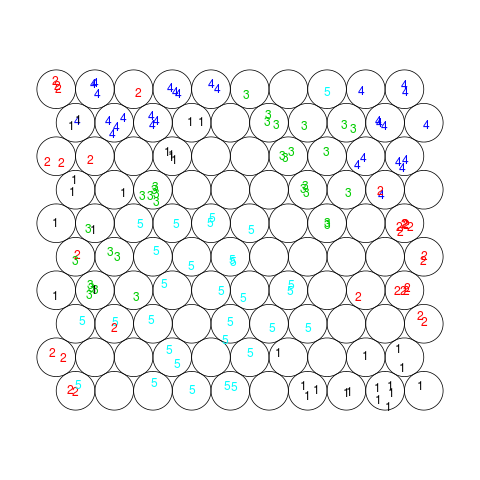
\includegraphics[width=0.45\textwidth]{../exps/som/sommultifractal}
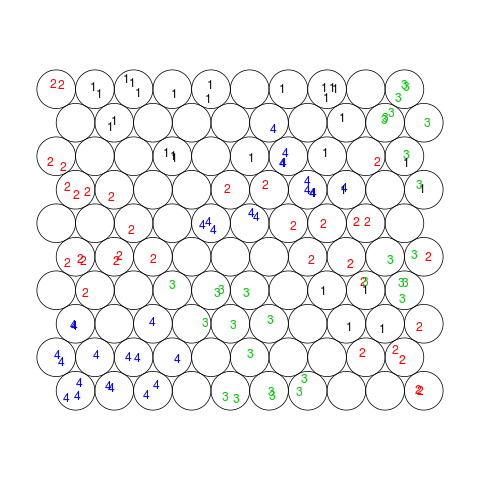
\includegraphics[width=0.45\textwidth]{../exps/som/sombreadmultifractal}
\caption{SOM of the bread and non-bread images (left) and SOM of the bread types only (right). $1$: {\em baguette}, $2$: {\em lactal}, $3$: {\em brun}, $4$: {\em sandwich}, $5$: {\em nonbread} }
\label{fig:somfractal}
\end{centering}
\end{figure*}

\begin{figure*}[htb]
\centering
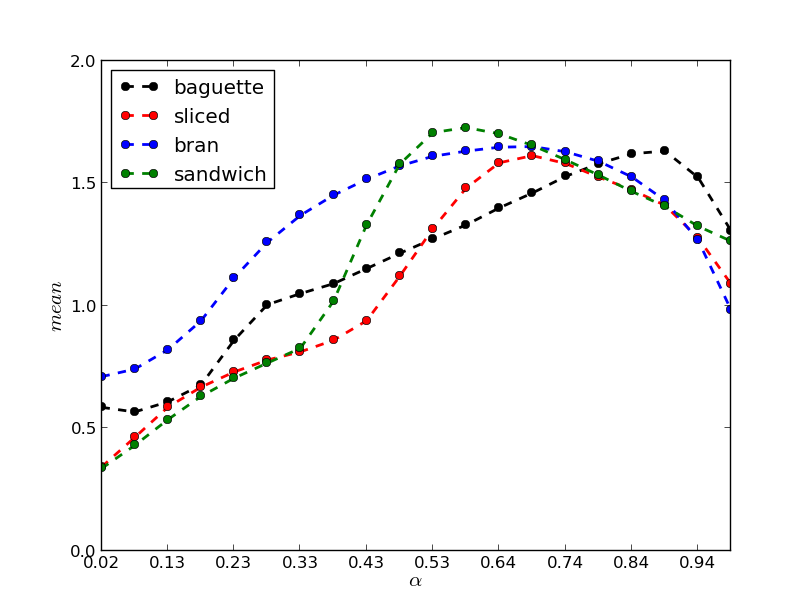
\includegraphics[scale=0.4]{../images/means}
\caption{Mean MFS for the four different bread types}
\label{fig:meansMFS}
\end{figure*}


In Figure \ref{fig:meansMFS}, the mean values of the MFS for the four different bread types are shown. This image shows, similarly to the SOM maps, that the MFS could potentially characterize and classify the different bread crumb types, since the mean values are different for each class. The standard deviations for the MFS of the different bread types are shown in Table \ref{fig:stdevMFS}. From the table, it can be seen that in the first half of the MFS (first $10$ FDs), the standard deviation of the FDs is higher than in the second half of the spectrum (last $10$ FDs). The spectrum in the last FDs tends to have a shape that identifies better a particular type of image. Usually, the spectrums of the same class and the same capturing method have, in this part of the spectrum, a shape that is useful to characterize the class. Nevertheless the capturing method and the illumination conditions of the image influences this shape, {\em i.e.} these two factors alters the MFS of the image. In other words, there is not an unique shape for each class of bread type.


\begin{figure*}[htb]
\centering
\includegraphics[scale=0.4]{../images/stdevTodos}
\caption{Standard Deviation for the FDs of the MFS for the four different bread types}
\label{fig:stdevMFS}
\end{figure*}


The correlation coefficients for the four bread types with the void fraction, mean cell area and standard deviation of mean cell area (in $mm^{2}$) are shown in Figures \ref{fig:corrVF}, \ref{fig:corrMCA} and \ref{fig:corrMCAstdev}, respectively. It is clear that the coefficients behave similarly for the first dimensions in all the bread types, but differently for the FD number \ and above. It could be concluded that the first dimensions are highly (negatively) correlated with the void fraction (porosity), mean cell area (coarseness) and the standard deviation of mean cell area (heterogeneity) of the bread types. It means that the first FDs increase when the mentioned features decrease. Other FDs also have a high (positive or negative) correlation, but it depends on the bread type which dimension is correlated.

From the graphs of the correlation coefficients of the VF, MCA and stCA, it could also be pointed out that the VF and the MCA have a higher correlation than the stCA with the FDs of the MFS. It means that the coarseness and the porosity of the bread crumb structure could be better determined by the features than its heterogeneity, using the MFS.

To summarise, the first half of the spectrum is useful to measure the porosity, coarseness and heterogeneity of the sample, while the second half of the MFS is useful to characterize the class of the image.



\begin{figure*}[htb]
\centering
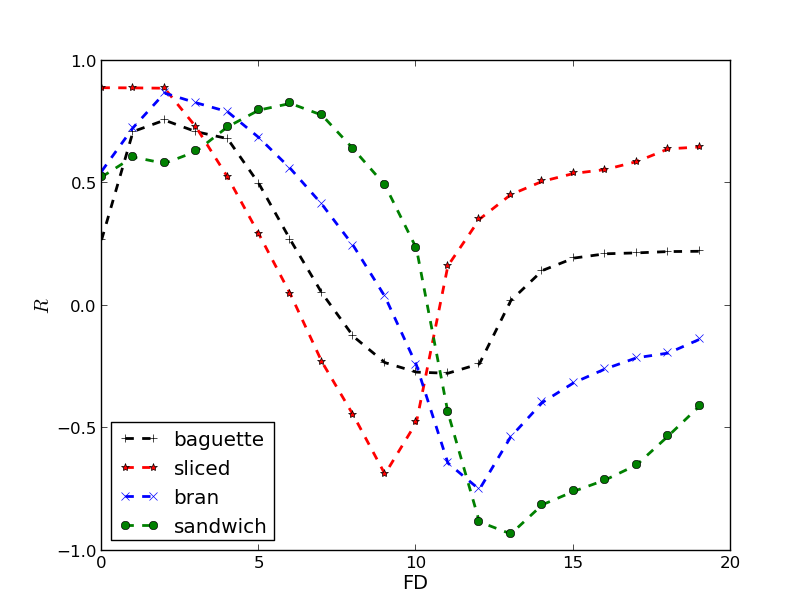
\includegraphics[scale=0.4]{../images/vf}
%\includegraphics[scale=0.3]{../images/vf105}
%\includegraphics[scale=0.3]{../images/vf40_105}
%\includegraphics[scale=0.3]{../images/vf40_110}
\caption{Correlation coefficients for the FDs and the void fraction of the samples}
\label{fig:corrVF}
\end{figure*}

\begin{figure*}[htb]
\centering
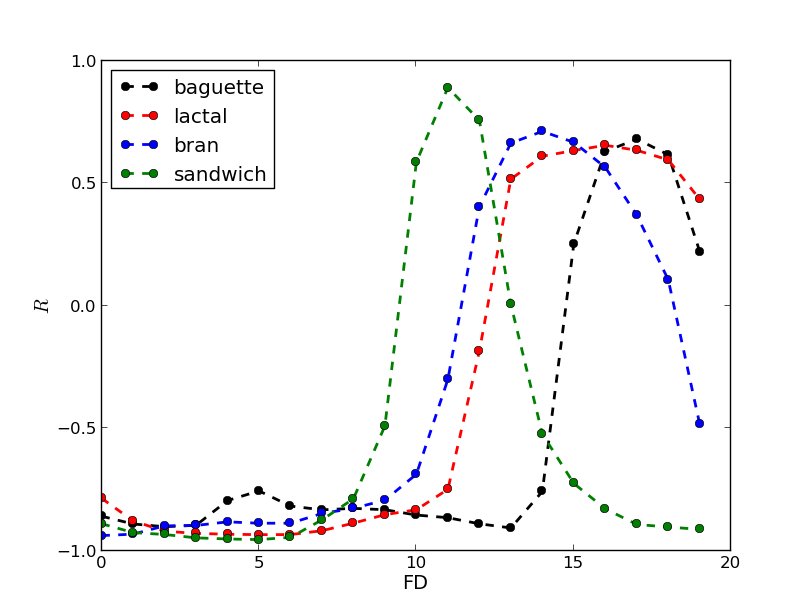
\includegraphics[scale=0.4]{../images/mca}
%\includegraphics[scale=0.3]{../images/mca105}
%\includegraphics[scale=0.3]{../images/mca40_105}
%\includegraphics[scale=0.3]{../images/mca40_110}
\caption{Correlation coefficients for the FDs and the mean cell area (in $mm^{2}$) of the samples}
\label{fig:corrMCA}
\end{figure*}

\begin{figure*}[htb]
\centering
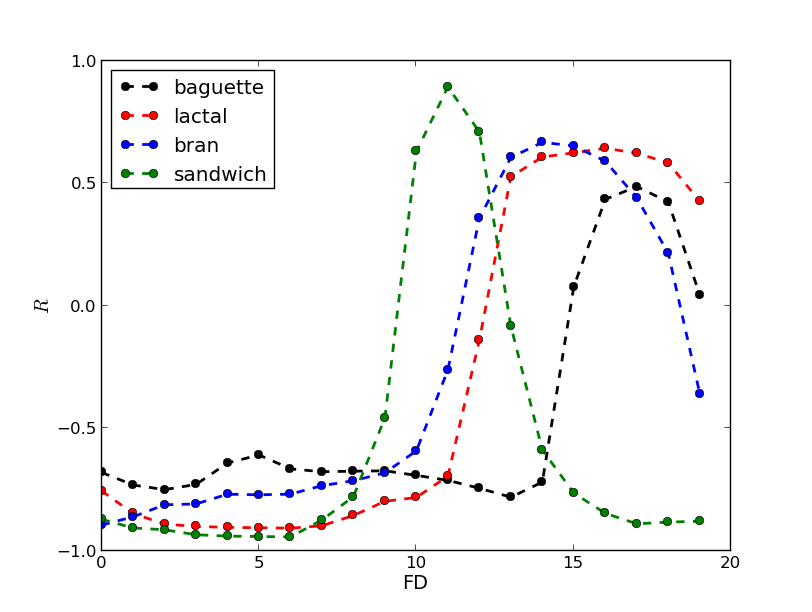
\includegraphics[scale=0.4]{../images/mcastdev}
%\includegraphics[scale=0.3]{../images/mcastdev105}
%\includegraphics[scale=0.3]{../images/mcastdev40_105}
%\includegraphics[scale=0.3]{../images/mcastdev40_110}
\caption{Correlation coefficients for the FDs and the standard deviation of the mean cell area (in $mm^{2}$) of the samples}
\label{fig:corrMCAstdev}
\end{figure*}

%\par\end{centering}

%\begin{centering}
%\subfloat[SOM using RGB features]{\begin{centering}
%\includegraphics[width=0.6\textwidth]{exps/som/som\mydot rgb}
%\label{fig:somrgb}
%\par\end{centering}
%}
%\par\end{centering}

%\caption{SOM of the scanned bread images (classes $1$~--~$4$) and the non bread images (class $5$)}


\subsection{Bread Classification}
\label{sec:10}

In order to test for the discriminative capability of the method, a classification experiment is made. Five classes are defined, {\emph e.g.}, {\emph baguette}, {\emph lactal}, {\emph bran}, {\emph sandwich} and {\emph non-bread}, assigning $40$ images to each class. A comparison is made between the MFS and state of the art features in the computer vision literature. This classification scheme is an intra-class one, and it is harder to solve than an ordinary inter-class one. 

K-fold cross validation is applied to the entire set (with $K=4$), employing three different classifiers: Support Vector Machines (SVM), Random Forests (RF), and Nearest Neighbors (NN). Results show that the MFS presents good classification performance regardless of the classifier employed. The libsvm implementation \cite{Chang2011} was used for the SVM classifier. In the case of the RF ($100$ trees) and the NN ($1$ neighbor) classifiers, the scikit-learn python library was employed.

In Table \ref{tab:number}, the classification performance of the method is tested using different numbers of FDs. When $20$ FDs are used, an useful combination of performance and low-dimensionality is achieved, so this number of FDs is used in the following calculations. The goal of this work is to show the impact of the features, rather than that of the classifier. The Nearest Neighbor results are considered the most relevant, since it shows the simplest classification rules among the three classifiers.

In Table \ref{tab:mfs}, several combinations of different MFS obtained from the images, and their classification performance are shown. The MFS used in the study were the density of the intensity (MFS in the table), the Laplacian of the intensity (L), and the gradient of the intensity (G). In addition, another test is made, using the CIELab color space. The key advantage of this color space is that it tends to reduce the dependency of the resulting image color on the dispositive used in the capture. The intensity of the images is transformed to the CIELab space, and the MFS of the three separated channels are combined together, obtaining a vector of $60$ FDs. This combination showed the best performance for the three classifiers. It means that adding color information in the $a$ and $b$ channels is useful for better classification of different types of bread crumbs, when different capturing dispositives are used (in this case, a scanner and a digital camera).

In Table \ref{tab:other}, state-of-the-art features (Haralick, Local Binary Pattern and SIFT features) are computed for the images. The best classification performance is obtained using the SIFT features, but it requires a $128$ feature length vector per image, and, in addition, it requires computational space and time to build internal structures. The classification performance of the MFS for the bread crumb database is the highest among the algorithms studied. The MFS captures robust and useful information for classification in low dimensional features. These results also agree with results obtained in \cite{Bosch2011} for the classification of other food products.

\begin{table}
% table caption is above the table
\caption{classification results with different number of FDs for the MFS}
\label{tab:number}       % Give a unique label
% For LaTeX tables use
\begin{tabular}{lllll}
\hline\noalign{\smallskip}
Number of FDs & 10  & 20 & 30 \\
\noalign{\smallskip}\hline\noalign{\smallskip}
SVM & \textbf{96\%} & 94.5\% & 95.5\% \\
RF  & 91.5\% & \textbf{93.5\%} & 93\% \\
NN & 88.5\% & \textbf{90.5\%} & 90\% \\
\noalign{\smallskip}\hline
\end{tabular}
\end{table}


\begin{table}
% table caption is above the table
\caption{classification results using different combinations of the MFS}
\label{tab:mfs}       % Give a unique label
% For LaTeX tables use
\begin{tabular}{lllll}
\hline\noalign{\smallskip}
Method & MFS & MFS+L & MFS+G & CIELab  \\
\noalign{\smallskip}\hline\noalign{\smallskip}
SVM & 94.5\% & 95.5\% & \textbf{97.5\%} & \textbf{97.5\%} \\
RF  & 93.5\% & \textbf{96\%} & 95\% & \textbf{96\%} \\
NN & 90.5\% & 90\% & 87\% & \textbf{92\%} \\
\noalign{\smallskip}\hline
\end{tabular}
\end{table}


\begin{table}
% table caption is above the table
\caption{classification results for different features}
\label{tab:other}       % Give a unique label
% For LaTeX tables use
\begin{tabular}{llllll}
\hline\noalign{\smallskip}
Method & Haralick & Lbp & SIFT\\ % & Zernicke
\noalign{\smallskip}\hline\noalign{\smallskip}
SVM & 94\% & 78.5\% & \textbf{96.5\%} \\ % & 55 
RF  & 91\% & 71.5\% & \textbf{92\%} \\ % & 58 
NN & 79\% & 70\% & \textbf{86\%} \\ % & 48.5 
\noalign{\smallskip}\hline
\end{tabular}
\end{table}




\section{Conclusions}
\label{sec:11}
The visual appearance of different types of bread crumbs can be successfully characterized by the fractal dimensions of its digital image. The first fractal dimensions obtained from the MFS method negatively measured bread crumb coarseness, porosity and heterogeneity, meaning that the lower the FD, the higher the measure. 


The use of multifractal features in bread crumb texture classification showed good performance. The MFS demonstrated to be accurate enough to perform a classification of different bread types and also to discriminate non bread from bread images. The classification performance of the MFS for the bread crumb database outperforms other state-of-the-art techniques employed in the computer vision literature. The information present in the MFS of the $a$ and $b$ channels of the CIElab space color provided the method with higher classification capabilities and obtained the best classification performance in all the developed tests. This result appear as a consequence of the different capturing dispositives used in this work. Also, it was shown that the MFS is sensitive to changes in the illumination conditions present in this work.

The results found can be applied to validate synthetic samples, {\em i.e.}, the latter should have similar features to the bread type that is trying to simulate. The features obtained will be used to determine particle system parameters ({\em e.g.}, particles lifetime, color, and also mean cell area, porosity and void fraction). These results can be extended to be used as quality parameters for these products.
%\begin{figure*}[htb]
%\centering
%$\vcenter{\hbox{\includegraphics[scale=1.3]{imagenes/salvado19}}}$
%$\vcenter{\hbox{\includegraphics[scale=0.4]{imagenes/fitbox}}}$
%\caption{An image and its computed box dimension}
%\label{fig:1}
%\end{figure*}

\begin{acknowledgements}
We would like to thank Gustavo Grieco and Pablo Speciale for technical discussions and for their support in the development of the present work. We would also like to thank Dra. Ursula Gonzales-Barron for the received images of bread crumbs.
\end{acknowledgements}

% BibTeX users please use one of
%\bibliographystyle{spbasic}      % basic style, author-year citations
%\bibliographystyle{spmpsci}      % mathematics and physical sciences
\bibliographystyle{spphys}       % APS-like style for physics
\bibliography{bibliografia/bibliografia}   % name your BibTeX data base

% Non-BibTeX users please use
%\begin{thebibliography}{}
%
% and use \bibitem to create references. Consult the Instructions
% for authors for reference list style.
%
%\bibitem{RefJ}
% Format for Journal Reference
%Author, Article title, Journal, Volume, page numbers (year)
% Format for books
%\bibitem{RefB}
%Author, Book title, page numbers. Publisher, place (year)
% etc
%\end{thebibliography}

\end{document}
% end of file template.tex

